\documentclass[12pt,oneside,a4paper]{book} % This style for A4 format.

%Packages
\usepackage{ecproject}
\usepackage{graphicx}
\usepackage{tikz}
\usetikzlibrary{calc}
\usepackage[a4paper, margin=1in]{geometry}
\usepackage{float}
\usepackage{qrcode}
%%%Page related
\usepackage{fancyhdr} % for header & footer
\usepackage[hidelinks]{hyperref}
\usepackage[toc, nonumberlist]{glossaries} %For Glossaries - to be loaded only after hyperref package
%\ifIndentPara
\usepackage{indentfirst}
%\fi
\usepackage{setspace}
%%%Table Related
%\usepackage{booktabs}
%\usepackage{makecell}
%\usepackage{multirow}
%\usepackage{multicol}


%Document settings
\title{Cell balancing for serially connected lithium-ion batteries}
%%%%%%%%%%%%%%%Minor (or) Major report%%%%%%%%%%%%%%%
%Uncomment \MinorProject line, if the report is for Minor project.
\MinorProject
%%%%%%%%%%%%%%%%%%%%%%%%%%%%%%%%%%%%%%%%%%%%%%
%%%Student Details%%%
\stuNameA{Shyamanth R H}
\stuUSNA{1RV17EC151}
\stuNameB{Amrathesh}
\stuUSNB{1RV17EC192}
%\stuNameC{Subrahmanya K N}
%\stuUSNC{1RV16EC007}

%%%Internal Guide%%%%
\guideNameA{Dr.Govinda Raju M}
\guideDesignationA{Assistant Professor}
\guideDeptA{Dept. of ECE}
\guideOrgA{RV College of Engineering}

%%%External Guide%%%%
%\guideNameB{Dr. Ramavenkateshwaran}
%\guideDesignationB{Assistant Professor}
%\guideDeptB{Dept. of ECE}
%\guideOrgB{RV College of Engineering}

%\guideNameC{Dr. Ramavenkateshwaran}
%\guideDesignationC{Assistant Professor}
%\guideDeptC{Dept. of ECE}
%\guideOrgC{RV College of Engineering}

\panelMemberA{Dr. Kariyappa}
\panelMemberDesigA{Professor}
\panelMemberB{Prof. P N Jayanthi}
\panelMemberDesigB{Assistant Professor}

\Department[ECE]{Electronics and Communication Engineering}

\HOD{Dr. K S Geetha}
\Principal{Dr. K. N. Subramanya}

\academicYear{2019-2020}

\QRurl{}
%\QRurl{https://drive.google.com/open?id=1jm-POmuq-ZZ1tT5m-xAdCDRnwvLZH8q-}
%%%%%%%%%%%%%%%%%%%For PG program%%%%%%%%%%%%%%%%%%%
%%%Uncomment \pgProgram command and define appropriate values for \MastersIn{} and \pgProgramName{}

%\pgProgram%
\MastersIn[M.Tech]{Master of Technology}
\pgProgramName{VLSI Design \& Embedded Systems}

%%%%%%%%%%%%%%%%%%Draft report%%%%%%%%%%%%%%%%%%
\DraftCopy
%%%%%%%%%%%%%%%%%%%%%%%%%%%%%%%%%%%%%%%%%%%%%%

%%%%%%%%%%%%%%%%%%Acronyms%%%%%%%%%%%%%%%%%%
\newglossary[sym]{symbolList}{sym1}{sym2}{List of Symbols}
\makeglossaries
%Acronyms
\loadglsentries{./AuxFiles/Glossaries}
\renewcommand{\glspostdescription}{}% To remove dot at the end
%%%%%%%%%%%%%%%%%%%%%%%%%%%%%%%%%%%%%%%%%%%%%%

%%%%%%%%%%%%%%Bibliography%%%%%%%%%%%%%%%%%%%%%
\usepackage[backend=biber,style=ieee]{biblatex}
%If backend is set to bibtex, then configure texmaker Bi(La)Tex with "bibtex %"
\addbibresource{./AuxFiles/ProjectBib.bib}%Add bib file with extention
%%%%%%%%%%%%%%%%%%%%%%%%%%%%%%%%%%%%%%%%%%%%%%

%%%%%%%%%%%%%%%%WaterMark%%%%%%%%%%%%%%%%%%%%%
%%Use it only after Biblatex
\usepackage[printwatermark]{xwatermark}
\newwatermark[allpages,color=gray!50,angle=0,scale=2,xpos=0,ypos=0]{
\includegraphics[width=0.3\textwidth]{Figures/RV_logoVecW}}
%%%%%%%%%%%%%%%%%%%%%%%%%%%%%%%%%%%%%%%%%%%%%%
\begin{document}
\maketitle
%\pagestyle{empty}
\newpage
\begin{spacing}{1.5}
%%ecproject package is created by P Narashimaraja, Assistant Professor, ECE, RVCE
%Border
\begin{tikzpicture}[remember picture, overlay]
  \draw[line width = 4pt] ($(current page.north west) + (0.75in,-0.75in)$) rectangle ($(current page.south east) + (-0.75in,0.75in)$);
\end{tikzpicture}
\thispagestyle{empty}
\vspace{-1cm}
\begin{center}
\Large\textbf{RV College of Engineering\textsuperscript{\small\textregistered}, Bengaluru} \par
\large{(\textit{Autonomous institution affiliated to VTU, Belagavi})} \par
\large\textbf{Department of \printDepartmentLF}\\
.\hspace{2cm}\\

\includegraphics[width=4cm]{Figures/RV_logoVec}\par
\Large\textbf{\underline{CERTIFICATE}} \par
\end{center}
%\begin{minipage}[b]{\linewidth}
%\large
\begin{spacing}{1.5}
\noindent Certified that the \ifMinor{minor\;}\else{ major\;}\fi project work titled \textbf{\textit{\printTitle}} is carried out by
\ifPG{%
\textbf{\printStuNameA} (\textbf{\printStuUSNA}) who is  bonafide student 
}
\else{ 
\ifStuNameCUsed{%
\textbf{\printStuNameA } (\textbf{\printStuUSNA}), \textbf{\printStuNameB } (\textbf{\printStuUSNB}) and \textbf{\printStuNameC } (\textbf{\printStuUSNC})  who are bonafide students 
}\else{%
\ifStuNameBUsed{%
\textbf{\printStuNameA} (\textbf{\printStuUSNA}) and \textbf{\printStuNameB} (\textbf{\printStuUSNB})  who are bonafide students 
}\else{%
\textbf{\printStuNameA} (\textbf{\printStuUSNA}) who is  bonafide student 
}
\fi
}\fi
}\fi
of RV College of Engineering, Bengaluru, in partial fulfillment of the requirements for the degree of  \ifPG \textbf{\printMastersInLF} in \textbf{\printMastersPrgName} \else\textbf{Bachelor of Engineering} in \textbf{\printDepartmentLF} \fi of the Visvesvaraya Technological University, Belagavi during the year \printAcadYear. It is certified that all corrections/suggestions indicated for the Internal Assessment have been incorporated in the \ifMinor{minor\;}\else{major\;}\fi project report deposited in the departmental library. The \ifMinor{minor\;}\else{ major\;}\fi project report has been approved as it satisfies the academic requirements in respect of \ifMinor{minor\;}\else{ major\;}\fi project work prescribed by the institution for the said degree.\\ \par
\end{spacing}

\begin{table}[H]
\centering
\resizebox{1\textwidth}{!}{%
\begin{tabular}{ccc}
\large Signature of Guide &\large Signature of Head of the Department &\large Signature of Principal\\
& &\\
\large\printGuideNameA & \large\printHOD & \large\printPrincipal\\
& & \\
\end{tabular}%
}
\end{table}

\begin{table}[H]
\centering
%\resizebox{\textwidth}{!}{%
\begin{tabular}{lccp{6cm}cc}
&&&\textbf{External Viva}&&\\
&&&&&\\
&Name of Examiners &&& & Signature with Date\\
&&&&&\\
1.&&&&&\\
&&&&&\\
2.&&&&&\\
\end{tabular}%
%}
\end{table}
%\pagebreak
\newpage
%%ecproject package is created by P Narashimaraja, Assistant Professor, ECE, RVCE
%%Border
\begin{tikzpicture}[remember picture, overlay]
  \draw[line width = 4pt] ($(current page.north west) + (0.75in,-0.75in)$) rectangle ($(current page.south east) + (-0.75in,0.75in)$);
\end{tikzpicture}

\thispagestyle{empty}

\begin{center}
\Large\textbf{\underline{DECLARATION}} \par
\end{center}


\noindent \ifPG I \else \ifStuNameBUsed We\else I\fi\fi, \textbf{\printStuNameA} \ifPG \else\ifStuNameBUsed , \textbf{\printStuNameB}$\,$ \ifStuNameCUsed and \textbf{\printStuNameC}$\,$ \fi \fi \fi students of \ifPG fourth \else \ifMinor{seventh\;}\else{eighth\;}\fi \fi semester \ifPG \printMastersInSF\, in \printMastersPrgName \else B.E.\fi, Department of \printDepartmentLF, RV College of Engineering, Bengaluru, hereby declare that the \ifMinor{minor\;}\else{ major\;}\fi project titled `\textbf{\printTitle}' has been carried out by \ifStuNameBUsed us \else me \fi and submitted in partial fulfilment for the award of degree of \ifPG \textbf{\printMastersInLF} in \textbf{\printMastersPrgName} \else\textbf{Bachelor of Engineering} in \textbf{\printDepartmentLF} \fi during the year \printAcadYear.\\ \par

\noindent Further \ifPG I \else\ifStuNameBUsed we \else I \fi \fi declare that the content of the dissertation has not been submitted previously by anybody for the award of any degree or diploma to any other university.\\ \par

\noindent \ifPG I \else\ifStuNameBUsed We \else I \fi \fi also declare that any Intellectual Property Rights generated out of this project carried out at RVCE will be the property of RV College of Engineering, Bengaluru and we will be one of the authors of the same.

\vspace{1cm}
\noindent Place: Bengaluru\par
\vspace{0.5cm}
\noindent Date: \par

\vspace{2cm}
\begin{table}[H]
\centering
%\resizebox{\textwidth}{!}{%
\begin{tabular}{llcp{5cm}cc}
&&&&&\\
&&&&&\\
&Name  &&& Signature& \\
&&&&&\\
1.&\printStuNameA (\printStuUSNA)&&&&\\
&&&&&\\
\ifPG% 
\else%
\ifStuNameBUsed%
2.&\printStuNameB (\printStuUSNB)&&&&\\
&&&&&\\
\else%
\fi%
\ifStuNameCUsed%
3.&\printStuNameC (\printStuUSNC)&&&&\\
&&&&&\\
\else%
\fi%
\fi%
\end{tabular}%
%}
\end{table}
%\pagebreak


\newpage
%%ecproject package is created by P Narashimaraja, Assistant Professor, ECE, RVCE.
%%Border
\begin{tikzpicture}[remember picture, overlay]
  \draw[line width = 4pt] ($(current page.north west) + (0.75in,-0.75in)$) rectangle ($(current page.south east) + (-0.75in,0.75in)$);
\end{tikzpicture}
\thispagestyle{empty}

\begin{center}
%.\hspace{1cm}\\ \par
\Large\textbf{\underline{ACKNOWLEDGEMENT}} \par
\end{center}

\ifPG I am \else
\ifStuNameBUsed We are \else I am \fi\fi indebted to \ifPG my \else\ifStuNameBUsed our \else my \fi\fi guide, \textbf{\printGuideNameA}, \printGuideDesigA, \printGuideOrgA$\,.$ for the wholehearted support, suggestions and invaluable advice throughout \ifPG my \else\ifStuNameBUsed our \else my \fi\fi project work and also helped in the preparation of this thesis.\\ \par

\ifPG I \else \ifStuNameBUsed We \else I \fi\fi also express our gratitude to \ifPG my \else\ifStuNameBUsed our \else my \fi\fi  panel members \textbf{\printPanelMemberA}, \printPanelMemberDesigA $\,$ and \textbf{\printPanelMemberB}, \printPanelMemberDesigB , Department of \printDepartmentLF\, for their valuable comments and suggestions during the phase evaluations. \\ \par

\ifPG My \else \ifStuNameBUsed Our \else My \fi\fi sincere thanks to \textbf{\printHOD}, Professor and Head, Department of \printDepartmentLF, RVCE for the support and encouragement.\\ \par

\ifPG I \else \ifStuNameBUsed We \else I \fi\fi express sincere gratitude to our beloved Principal, \textbf{\printPrincipal} for the appreciation towards this project work.\\ \par

\ifPG I \else\ifStuNameBUsed We \else I \fi\fi thank all the teaching staff and technical staff of \printDepartmentLF\, department, RVCE for their help.\\ \par 

Lastly, \ifPG I \else\ifStuNameBUsed we \else I \fi\fi take this opportunity to thank \ifPG my \else\ifStuNameBUsed our \else my \fi\fi family members and friends who provided all the backup support throughout the project work.\\ \par

%\pagebreak
\newpage
\pagenumbering{roman}
\chapter*{Abstract}

\addcontentsline{toc}{chapter}{Abstract}\vspace{-1cm}
%Border
\begin{tikzpicture}[remember picture, overlay]
  \draw[line width = 4pt] ($(current page.north west) + (0.75in,-0.75in)$) rectangle ($(current page.south east) + (-0.75in,0.75in)$);
\end{tikzpicture}


Growing concerns on climate change and global warming, world as already started looking for eco-friendly alternatives in every domain possible and most of these alternatives use electricity to power up the system which adds in batteries and by virtue batteries are costly needs to be properly maintained. A weak cell in the battery pack will charge and discharge faster than  higher capacity cells and thus it becomes the limiting factor in the run-time of a system. Cell balancing circuits are very necessary in every \acrfull{bms} to equalize cell \acrfull{soc}  so that pack delivers its rated capacity. Passive balancing technique is a simple and low-cost method to equalize the \acrshort{soc} of cells in a battery pack. 

The objective of this project is to develop a passive cell balancing module using cell monitoring \acrshort{ic} BQ76PL455A-Q1 and STM32F103C8T6 microcontroller. A MATLAB\textsuperscript{\textregistered} Simulink\textsuperscript{\textregistered} model of battery pack is designed to aid development of an efficient cell balancing algorithm and to validate its working. Stateflow\textsuperscript{\textregistered}, a Simulink\textsuperscript{\textregistered} add-on is used to develop logic and visualize the algorithm on the run.

A passive cell balancing module based on  BQ76PL455A-Q1 \acrshort{ic} is designed using KiCAD, an open-source PCB design software. STM32F103C8T6 microcontroller was used to run the algorithm, sample cell voltages and perform balancing for a battery pack consisting of 6 cells in series. The module is capable of supporting upto 16 cells in series and can be integrated with Battery management system of Li-ion battery pack with ease. The simulation which was made to validate the balancing algorithm was run for 15 hours and after 6 charge-discharge cycles an imbalanced battery pack got balanced by the application of balancing algorithm. 
 
\pagebreak 
\end{spacing}
\newpage
\pagestyle{fplain}
\begin{spacing}{1.5}
	\tableofcontents	
\end{spacing}
\newpage
\begin{spacing}{1.5}
	\cleardoublepage
	\addcontentsline{toc}{chapter}{\listfigurename}
	\listoffigures	
\end{spacing}
\newpage
\begin{spacing}{1.5}
	\cleardoublepage
	\addcontentsline{toc}{chapter}{\listtablename}
	\listoftables	
\end{spacing}
\newpage
\printglossary[type=\acronymtype, title= Abbreviations, toctitle=Abbreviations]
\newpage
\printglossary[type=symbolList, title= List of Symbols, toctitle=List of Symbols]

\mainmatter
\pagestyle{mplain}
\glsresetall
\begin{spacing}{1.5}
%Chapter 1 
\chapter{Introduction to Analog and Digital converters}
Every chapter should start with an introduction paragraph. This paragraph should brief about the flow of the chapter. This introduction can be limited within 4 to 5 sentences. The chapter heading should be appropriately modified (a sample heading is shown for this chapter).
\section[Introduction]{\textbf{Introduction}}
The title of the project can be introduced in this section. This section should neatly elaborate the context of the project, the relevance of the area chosen and the title. You can bring a brief history and arrive at the title of the project. Use appropriate number of paragraphs within this section. 

You are allowed to use figures or diagrams which can help in introducing the topic acknowledging the source. For example , if you are introducing a particular topic, an appropriate figure can be used. The figure should be referenced in the text as Figure. \ref{fig:universe} 
\begin{figure}[htb]
\centering
	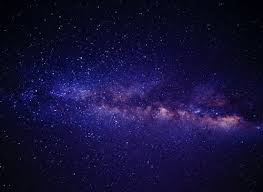
\includegraphics[scale=1]{Figures/universe}	
	\caption{Sample picture of universe }
	\label{fig:universe}
\end{figure}

These guidelines are provided to formally expose you to the various ethical and technical issues involved in writing up your work and the format you are required to adhere to while submitting your project report.

\section[Motivation]{\textbf{Motivation}}

Brief the motivation of selecting your project title. You can elaborate the challenges in the specific area, relevance and importance of the chosen topic. 

\section[Problem statement]{\textbf{Problem statement}}

Define the problem statement in this section, in one paragraph.

\section[Objectives]{\textbf{Objectives}}
The objectives of the project are
\begin{enumerate}
\item To design a pipelined ADC for audio frequency range
\item List all the objectives in the above format , starting with "To"
\item Limit the number of objectives to a maximum of three
\end{enumerate}

\section[Literature Review]{\textbf{Literature Review}}

A literature review is a text of a scholarly paper, which includes the current knowledge including substantive findings, as well as theoretical and methodological contributions to a particular topic. Literature reviews are secondary sources, and do not report new or original experimental work. Most often associated with academic-oriented literature, such reviews are found in academic journals, and are not to be confused with book reviews that may also appear in the same publication. Literature reviews are a basis for research in nearly every academic field . A narrow-scope literature review may be included as part of a peer-reviewed journal article presenting new research, serving to situate the current study within the body of the relevant literature and to provide context for the reader. In such a case, the review usually precedes the methodology and results sections of the work.

\subsection{Sample}
The main types of literature reviews are: evaluative, exploratory, and instrumental. A fourth type, the systematic review, is often classified separately, but is essentially a literature review focused on a research question, trying to identify, appraise, select and synthesize all high-quality research evidence and arguments relevant to that question. A meta-analysis is typically a systematic review using statistical methods to effectively combine the data used on all selected studies to produce a more reliable result.
\subsubsection[Review types]{\textbf{Review types}}

The main types of literature reviews are: evaluative, exploratory, and instrumental. A fourth type, the systematic review, is often classified separately, but is essentially a literature review focused on a research question, trying to identify, appraise, select and synthesize all high-quality research evidence and arguments relevant to that question. A meta-analysis is typically a systematic review using statistical methods to effectively combine the data used on all selected studies to produce a more reliable result.


\subsubsection[Process and product]{\textbf{Process and product}}

Distinguish between the process of reviewing the literature and a finished work or product known as a literature review. The process of reviewing the literature is often ongoing and informs many aspects of the empirical research project. All of the latest literature should inform a research project. Scholars need to be scanning the literature long after a formal literature review product appears to be completed.

\subsubsection{\textbf{Page limitation}}

A careful literature review is usually 15 to 30 pages and could be longer. The process of reviewing the literature requires different kinds of activities and ways of thinking and link the activities of doing a literature review with Benjamin Bloom’s revised taxonomy of the cognitive domain (ways of thinking: remembering, understanding, applying, analysing, evaluating, and creating).

This section should contain the review of the literature in the past.You should review a minimum of 10 papers from standard reference journals. Kindly avoid local conference papers and papers from predatory journals. Kindly consult with your guide and finalize papers to be considered for review before adding in this section.Report the major observations and findings from each paper in one paragraph in the format given below.

 proposed various techniques for adders and multipliers.Add the reference papers to the bibliography section using Jabref and cite it here using the instructions given in further chapters.


\subsubsection{\textbf{Plagiarism}}

To use someone else's exact words without quotation marks and appropriate credit, or to use the unique ideas of someone else without acknowledgement, is known as plagiarism. In publishing, plagiarism is illegal; in other circumstances, it is, at the least, unethical. You may quote or paraphrase the words or ideas of another if you document your source. Although you need not enclose the paraphrased material in quotation marks, you must document the source. 

Paraphrased ideas are taken from someone else whether or not the words are identical. Paraphrasing a passage without citing the source is permissible only when the information paraphrased is common knowledge in a field. (Common knowledge refers to historical, scientific, geographical, technical, and other type of information on a topic readily available in handbooks, manuals, atlases and other references). 

\subsubsection{How to add Reference}
Use \texttt{Jabref} which will help in adding the reference in a separate file, from which one can use \verb|\citep\{\}| command to add reference. A sample, referring to a textbook would look something like this,\cite{Razavi2000}.

\section[Brief Methodology of the project]{\textbf{Brief Methodology of the project}}
Discuss about the methodology you identified to execute the objectives of your project in brief. Methodology is a system of practices, techniques, procedures, and rules used to execute a particular project. You can elaborate the methodology in a later chapter. Here you can present in the form of a flow diagram and explain the methodology in a paragraph.

\section[Assumptions made / Constraints of the project]{\textbf{Assumptions made / Constraints of the project}}

List the assumptions made for the execution of the project in this section. You can also elaborate on the major constraints of the project. This section should clearly state under what conditions your project is valid. It is mandatory to have this section in your project report.

\section[Organization of the report]{\textbf{Organization of the report}}

This report is organized as follows. Write the discussions in each chapter. A sample is as follows.
\begin{itemize}
\item Chapter 2 discusses the fundamentals of ADC and the performance parameters for evaluation.
\end{itemize}

In a similar way, write briefly about each chapter in one or two sentences.

%Chapter 2
\chapter{Theory and Fundamentals of Analog to Digital converter}

Every chapter should start with an introduction paragraph. This paragraph should brief about the flow of the chapter. This introduction can be limited within 4 to 5 sentences. The chapter heading should be appropriately modified (a sample heading is shown for this chapter). 
\section{Contents of this chapter}

This chapter should discuss about the prerequisite learnings before the execution of the project. Organise and elaborate the theory and necessary fundamentals required for the execution of the project. You can use \verb|\subsections| and \verb|subsubsections| in this chapter.
\section{Contents of this chapter}
If a specific programming language is required for the project, a section can be allotted in this chapter to discuss it. 
\section{Contents of this chapter}
Tools used could be another possible section to discuss about the software tools used in the work. 
\section{Contents of this chapter}
The details in this chapter can be added in consultation with the project guide. For an internship based projects, subsections can be modified accordingly. 

\section{Use of Acronyms and Glossaries}
Acronyms are nothing but the short form of regular repeated word. Say for example, you have a repeat word "Integrated Circuits" and you want to use a short form for it as "IC". For which you have to first define the word and use it wherever you wanted to refer it.

First, let's look at the definition, which has to be entered in \texttt{Glossaries.tex} under \texttt{CoverPages} directory.
\begin{verbatim}
%\newacronym{<Ref>}{<Short-Form>}{<Expanded word>}
\newacronym{ic}{IC}{Integrated Circuits}
\end{verbatim}
In order to use the defined acronym, use the commands \verb|\gls{<Ref>}| as shown below

As an example, call the definition with \verb|\gls{ic}| and the outcome of it is reflected as, \gls{ic}.

Note: For the First time, the expanded form appears along with the Short-form definition inside parenthesis. But when the \verb|\gls{}| is repeated, only Short-form appears inside the parenthesis.

Now, let's look at the definition of symbols. Follow the syntax to define the symbol first, inside \texttt{Glossaries.tex} under \texttt{CoverPages} directory.
\begin{verbatim}
%\newglossaryentry{<Ref>}{name=<Symbol>, description={<description about the symbol>}, type=<List type>}
\newglossaryentry{rc}{name=$\tau$, description={Time constant}, type=symbolList}
\end{verbatim}

As an example, the rate of change is defined with \verb|\gls{rc}| and the outcome of it is reflected as, the rate of change is defined with \gls{rc}.

\vspace{0.75cm}

After elaborating the various sections of the chapter, a summary paragraph should be written discussing the highlights of that particular chapter. This summary paragraph should not be numbered separately.  


%Chapter 3
\chapter{Design and Development of Cell Balancing Circuit}

\indent\indent In this chapter design and development of cell balancing circuit and methods followed in development and testing of  the balancing algorithm in MATLAB\textsuperscript{\textregistered} Simulink\textsuperscript{\textregistered} environment is discussed. 


\section{Cell Calancing Circuit}
As discussed in Chapter 2, switching shunt resistor method is used for the design. In which highest SOC cell is discharged through a shunt resistance and the discharging is controlled with \acrshort{mosfet} as shown in the Figure 3.1. A diode is connected in series with resistance to avoid any reverse current during charging of battery pack.

\begin{figure}[h!]
    \centering
    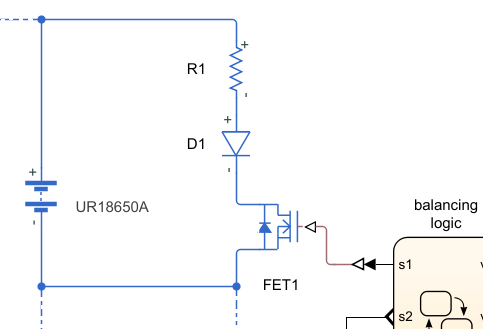
\includegraphics[]{Chapter3/Figures/cell_bal_ckt.PNG}
    \caption{Switched shunt cell balancing circuit}
\end{figure}

\subsection{Bleed Resistor}
The value of bleed resistor chosen on the basis of percentage of time the cell balancing circuit is enabled and the delta leakage current. Since this balancing circuit is meant for an \acrshort{ev} keeping power saving in mind an assumption that \acrshort{bms} will be ON for 20 percent of the time is made.

Depending on the time available for balancing and capacity of the battery pack the balancing current need to be decided. Since, BQ76PL455A \acrshort{ic} can support up to 16 Li-ion cells which is nearly 4Ah, after referring balance time versus balance current graph shown in Fig 3.2 a balancing current of 200 mA is chosen for the design. So the circuit will be able to balance the battery pack in about 10 hours in worst case i.e when the pack has some cells fully charged and some cells are near empty.

\vspace{0.5cm}

\begin{figure}[h!]
    \centering
    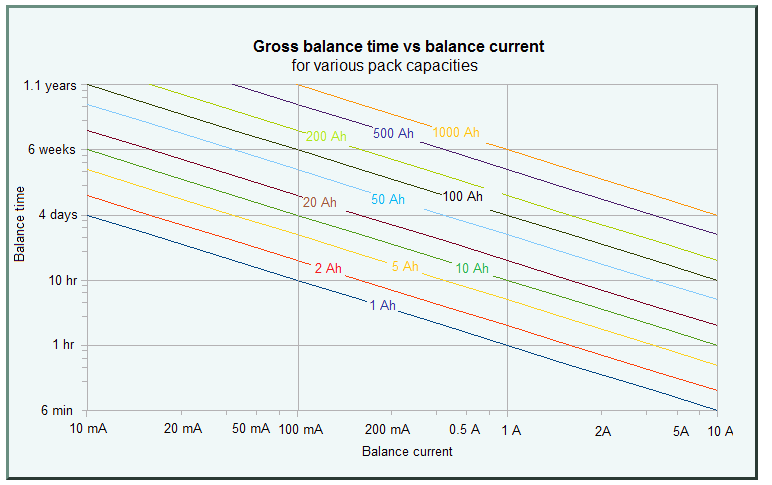
\includegraphics[scale = 0.72]{Chapter3/Figures/balcurrent_graph.PNG}
    \caption{Balancing time versus balance current graph taken from \cite{wpbalcur} }
\end{figure}

From UR18650 Li-ion cell datasheet nominal cell voltage $V = 3.7V$ and balancing current $I= 200 mA$. Using Ohm's law,

\[ V = IR\]
\[ R = \frac{V}{I}\]
\[ R = \frac{3.7}{200 *10^-^3}\]
\[ R = 18.5 \Omega\]

\subsection{Schematic of cell balancing circuit}
A MATLAB\textsuperscript{\textregistered}-Simulink\textsuperscript{\textregistered} model is developed for a battery containing 3 cells. For each cell a parallel balancing path is provided and a \acrshort{mosfet} is used to control cell discharging for balancing purpose. The state of each \acrshort{mosfet} in the design depends on the balancing logic block output as shown in Figure 3.3.

\begin{figure}[h!]
    \centering
    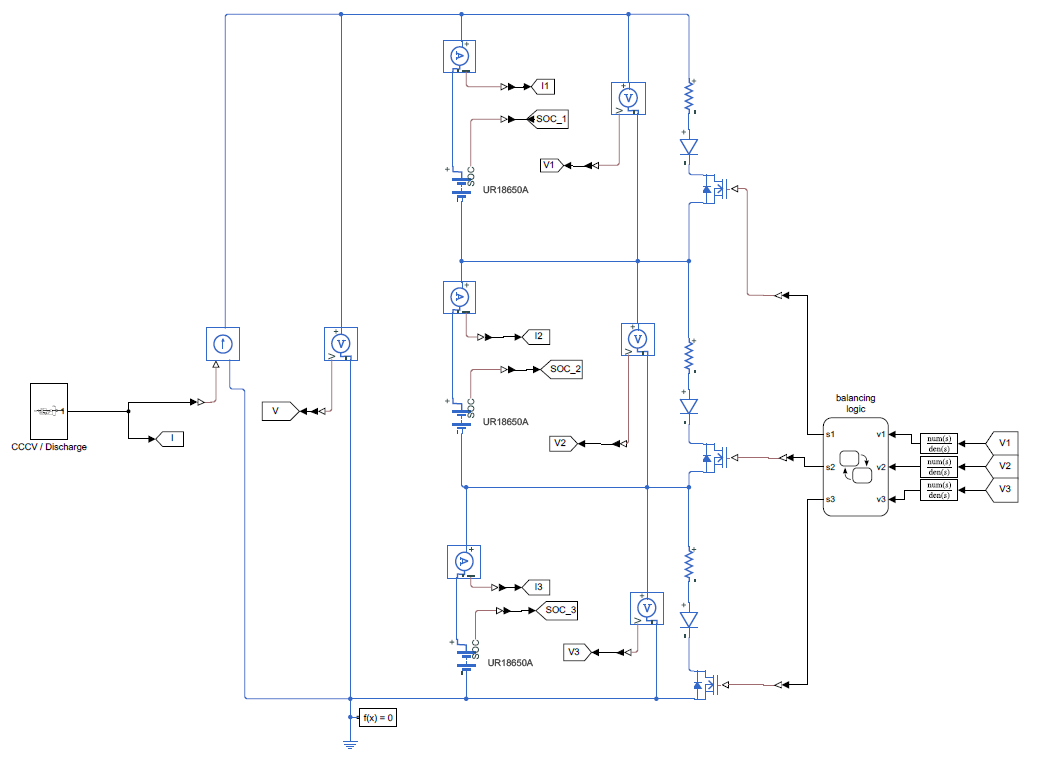
\includegraphics[scale = 0.6]{Chapter3/Figures/mainmodel.PNG}
    \caption{MATLAB\textsuperscript{\textregistered}-Simulink\textsuperscript{\textregistered} model to simulate passive cell balancing}
\end{figure}

\subsection{Simscape™}
Simscape™ is physical modelling add-on for Simulink\textsuperscript{\textregistered} environment. It provides battery cell models with other physical components like diode,resistor etc. which are designed by application engineers using physical data sets, so these models are very close to real hardware and gives good simulation results.

Panasonic UR18650 Li-ion cell model from Simscape™ Library is used for Simulink\textsuperscript{\textregistered} model. The cell model works based on look-up tables and user has freedom to override parameters like initial SOC level of cells, cell voltages etc as shown in figure 3.4.

\begin{figure}[h!]
    \centering
    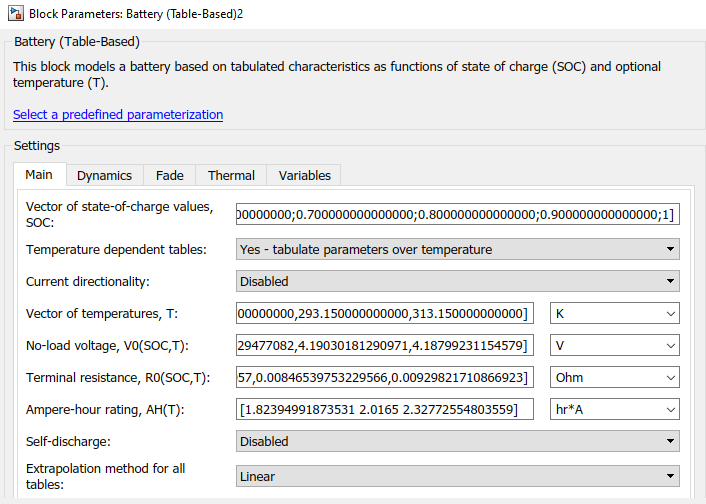
\includegraphics[scale = 0.72]{Chapter3/Figures/battery_model.PNG}
    \caption{Look up table of Simscape™ UR18650 cell model }
\end{figure}

\section{Cell balancing algorithm }
\subsection{Balancing Logic}
To perform passive cell balancing individual cell voltages or SOCs are sampled to decide which cell has to discharged via bleed resistor. The algorithm uses cell voltages to make decisions since it is easy to measure cell voltages rather then estimating individual cell's state of charge. When difference of minimum and maximum cell voltage becomes greater than 0.01V the battery pack is said to be imbalanced and it is left to the designer to choose this voltage difference value depending on extent of balancing required. The Figure 3.5 shows flowchart representation of the algorithm.

\begin{figure}[H]
    \centering
    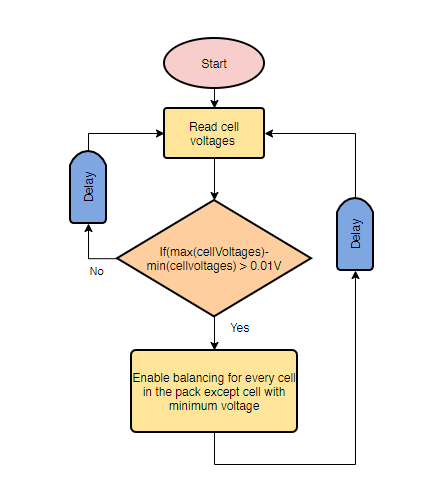
\includegraphics[]{Chapter3/Figures/logic.PNG}
    \caption{Balancing Logic flowchart}
\end{figure}

\subsection{Stateflow\textsuperscript{\textregistered}}
Stateflow\textsuperscript{\textregistered} is logic tool used to model systems using state machines and flow charts in Simulink\textsuperscript{\textregistered} environment. During simulations state switching can be visualised and debugging is made easy so that potential bugs are eliminated in early stages. Using Hardware Support packages code can be generated using Embedded code generator and it also provides options to generate code which is compliant with industry standards.



\begin{figure}[H]
    \centering
    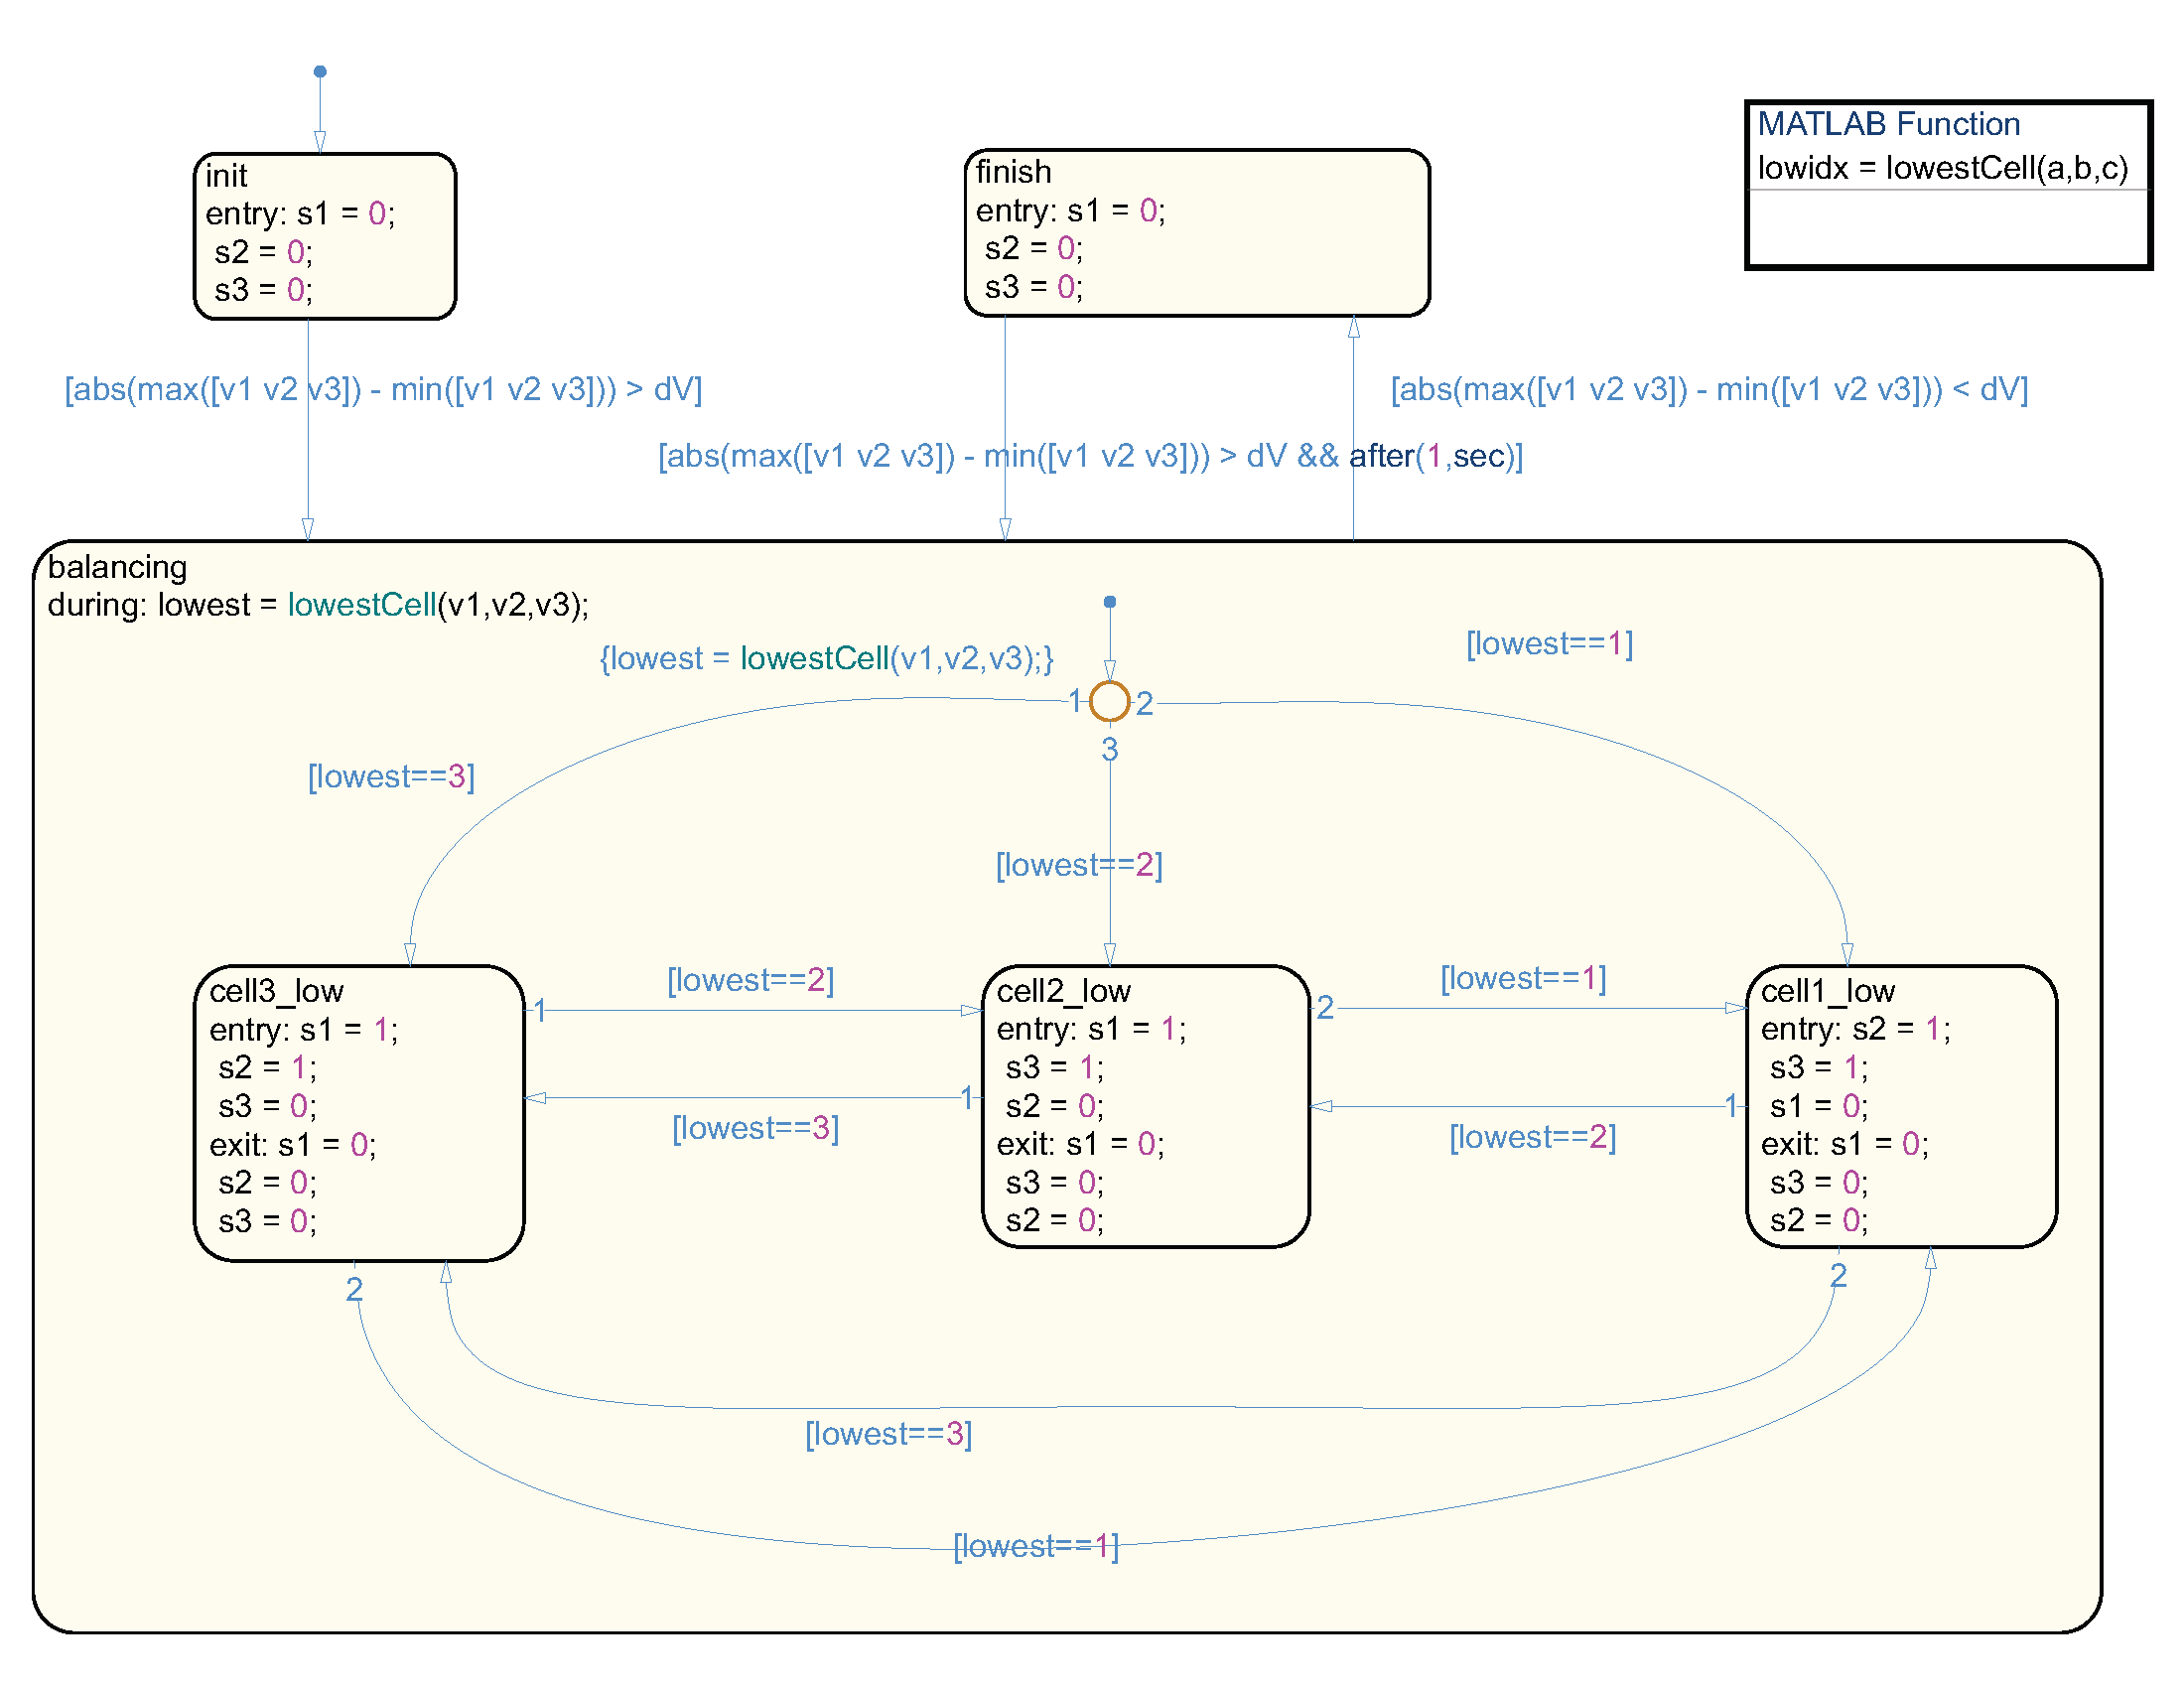
\includegraphics[scale = 0.6]{Chapter3/Figures/balancing logic.png}
    \caption{State machine for cell balancing in Stateflow\textsuperscript{\textregistered}}
\end{figure}


The logic represented in flowchart is reproduced in Stateflow\textsuperscript{\textregistered} as a state machine. The Stateflow\textsuperscript{\textregistered} diagram of the balancing logic is shown in Figure 3.6.

\vspace{1cm}

In this chapter, the details of design and development of cell balancing circuit and simulation of balancing algorithm in Simulink\textsuperscript{\textregistered}-Matlab\textsuperscript{\textregistered} is discussed. The results obtained during simulation validates the balancing algorithm. In the next chapter, implementation of balancing circuit on printed circuit board is discussed.

%Chapter 4
\chapter{Implementation of Pipelined Analog to Digital converter}

\indent\indent Every chapter should start with an introduction paragraph. This paragraph should brief about the flow of the chapter. This introduction can be limited within 4 to 5 sentences. The chapter heading should be appropriately modified (a sample heading is shown for this chapter). 

\section{Contents of this chapter}
This chapter should elaborate the following in detail.
\begin{enumerate}
\item Implementation details for hardware based projects
\item Top level Design for software based projects
\end{enumerate}

You can add sections and sub sections to elaborate your project work done.

\vspace{0.75cm}

After elaborating the various sections of the chapter, a summary paragraph should be written discussing the highlights of that particular chapter. This summary paragraph should not be numbered separately.  



%Chapter 5
\chapter{Results \& Discussions}
\indent The results obtained from the cell balancing module and the MATLAB Simulink model are presented in form of graphs and figures. And observations made during testing are discussed in the chapter.



\section{Simulation results}
Initially the cells in pack are set at random SOC values so that pack is said to imbalanced. Simulation time is set for 15 hours and run in rapid accelerator mode in Simulink.


\begin{figure}[h!]
    \centering
    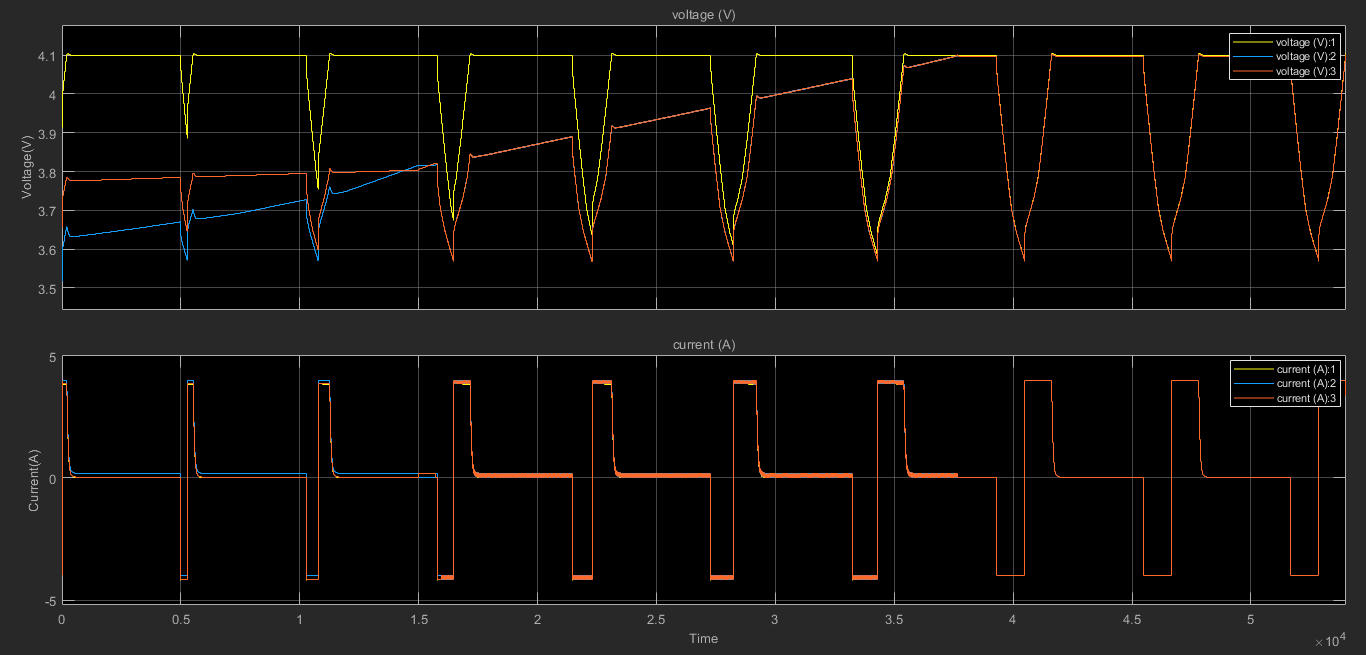
\includegraphics[scale = 0.5]{Chapter5/Figures/cellsVI.png}
    \caption{Cell voltage and current versus time during charge-discharge cycles}
\end{figure}

Fig 5.1 shows cell voltage and current versus time graph during charge-discharge cycles.Initially when battery pack is imbalanced the lowest voltage cell was limiting battery's full capacity even though other cells had charge remaining because of \acrshort{bms} cutting off discharge when one of the cell in pack reaches lowest set cell voltage in order to protect cells from  damage. As cell balancing algorithm kicks in cell voltages equalise and after 6 charge-discharge cycles the battery pack get balanced and deliver the rated capacity.
\vspace{0.5cm}
\begin{figure}[h!]
    \centering
    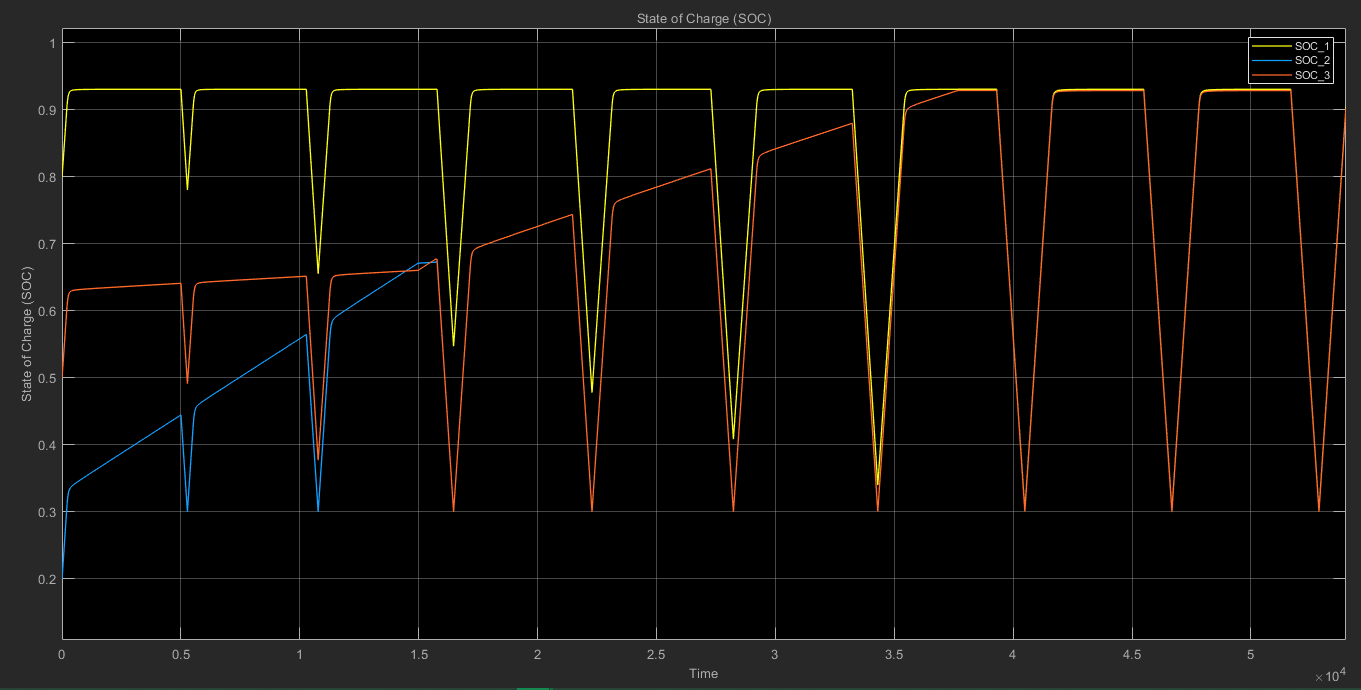
\includegraphics[scale = 0.5]{Chapter5/Figures/soc.png}
    \caption{State of charge of cells versus time during charge-discharge cycles}
\end{figure}

Figure 5.2 shows state of charge of cells versus time graph during charge-discharge cycles. Again it validates the circuit as by reporting full capacity utilisation after balancing circuit gradually equalise cell voltages.

\begin{figure}[h!]
    \centering
    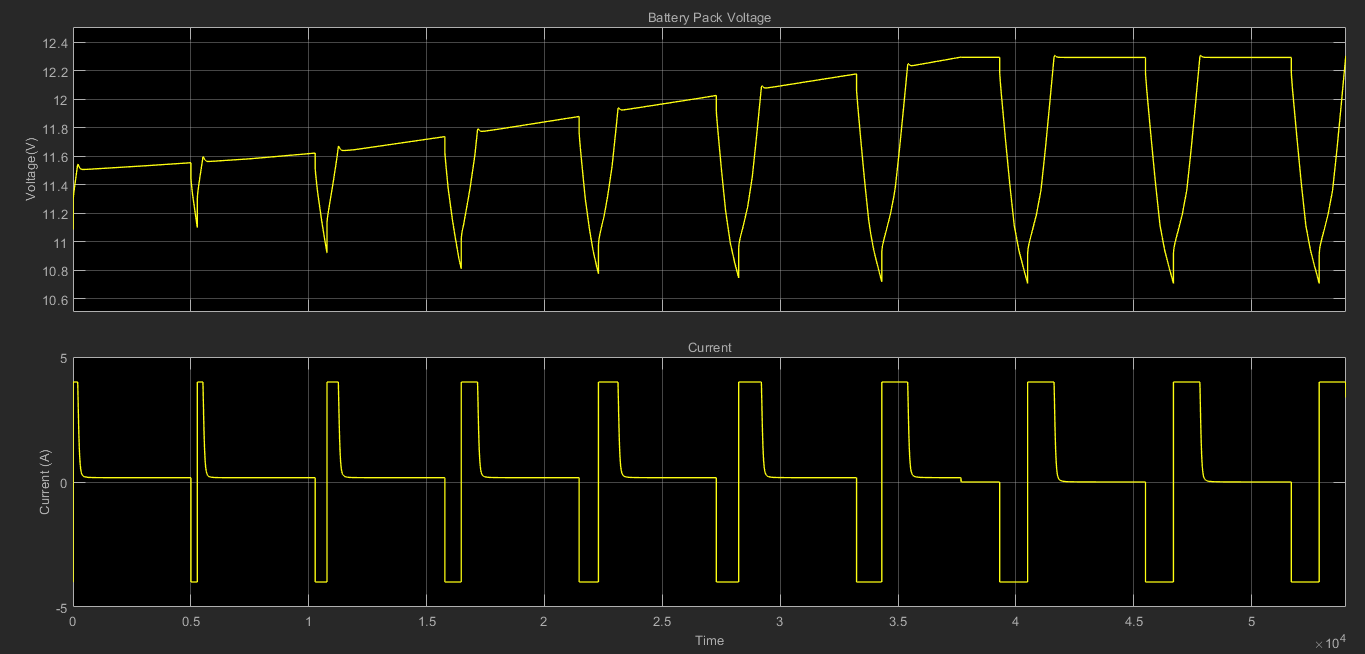
\includegraphics[scale = 0.5]{Chapter5/Figures/batterypackvoltage.png}
    \caption{Battery pack voltage and current versus time during charge-discharge cycles}
\end{figure}
\vspace{0.5cm}
Figure 5.3 shows battery pack voltages before and after balancing so it gives an observation that imbalanced circuit will not only affect the effective capacity of battery but also the terminal voltage of the battery pack. And a increase of nearly 0.6V is observed after battery got balanced by the circuit.

\pagebreak

\section{Cell balancing module test results} 
The debugging of the circuit is done using ST-Link Debugger with Keil. And data transaction between the battery monitoring \acrshort{ic} and the microcontroller is monitored in order to verify whether the module and code is working as expected. 

\begin{figure}[H]
    \centering
    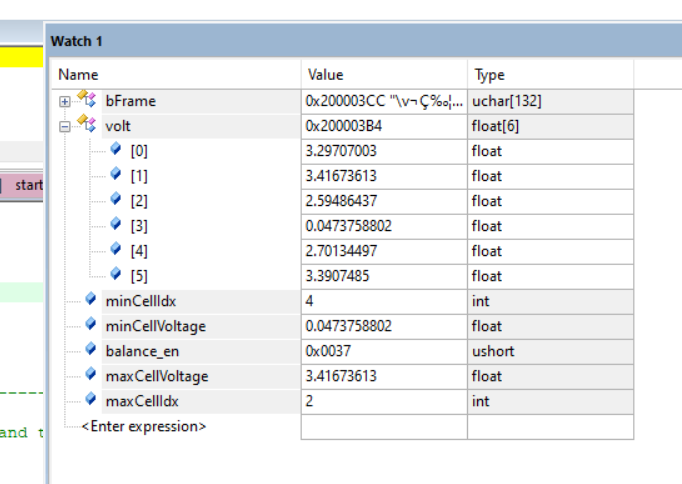
\includegraphics[scale = 0.7]{Chapter5/Figures/Screenshot (68).png}
    \caption{Battery pack voltage readings with minimum and maximum cell voltages}
\end{figure} 

Figure 5.4 shows the watch point in Keil IDE showing all the cell voltages in the battery pack with minimum and maximum cell voltage. 



%Chapter 6
\chapter{Conclusion and Future Scope}

\section{Conclusion}
This chapter should not contain an introduction paragraph like other chapters. You can directly write conclusion of the work done under this section. Typically this section can have 3 to 4 paragraphs. 

First paragraph should bring in the scenario of the project and every objective should be explained here.

Second paragraph should say how the objectives are implemented and achieved.

Last paragraph should draw the conclusions from each objective with quantitative results, performance improvement etc. 

\section{Future Scope}
Briefly discuss the constraints and limitations of the project and state the possibilities of extending the work in future.
\section{Learning Outcomes of the Project}
\begin{itemize}
\item List the learning outcomes here
\item List a minimum of 5 learning outcomes
\end{itemize}



\backmatter
\clearpage
%\ifDrft{
%%Do Nothing
%}\else{
\printbibliography%
%}
%\printindex
\end{spacing}
\end{document}